\newpage

\section{Actividad 2: Estrangulamiento del Canal $V_{GS(off)}$}

\subsection{Simulación}

Para la siguente simulacion añadiremos una fuente que varía de 0 a 7 en polarizaión inversa a la compuerta para extrangular el canal, obteniendo el siguiente circuito:

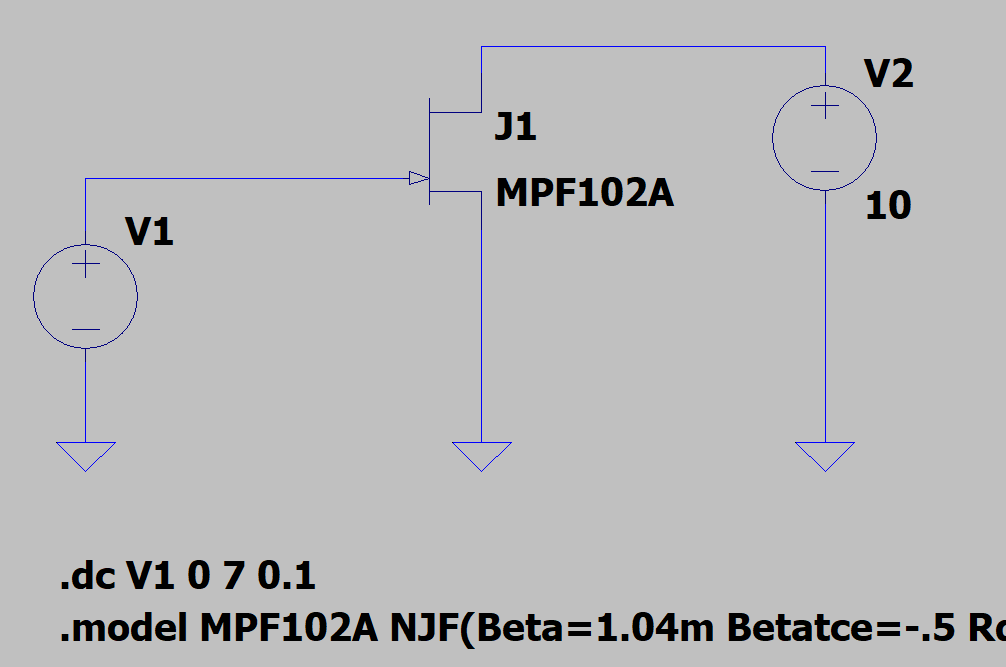
\includegraphics[width=6cm]{./imagenes/Circ2.png}

Al simularlo se obtiene la siguiente gráfica:

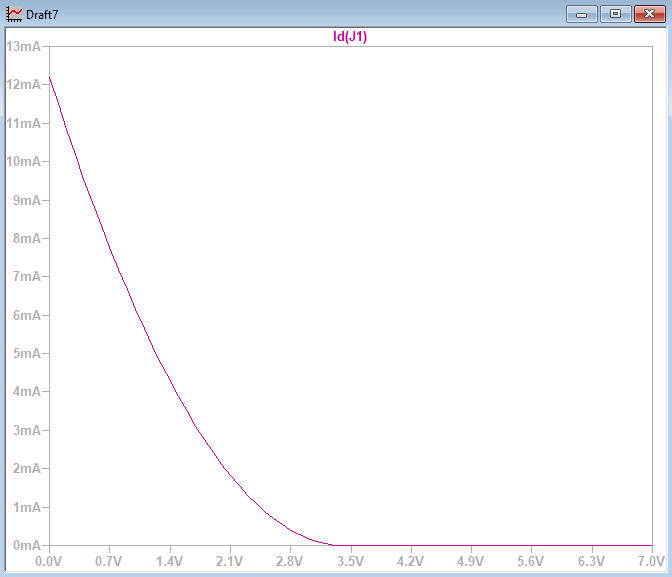
\includegraphics[width=8cm]{./imagenes/Sim2.png}

En ella observamos El valor $I_{DSS}$ de la simulación anterios rondando los 12mV, y ademas obtenemos un nuevo valor, el cual es $V_{GS(off)}$ que en nuestro caso es de -3,3V.

\subsection{Laboratorio}

\paragraph{Instrumental y Materiales}
\begin{itemize}
    \item Multimetro UNI-T UT89X
    \item Transistor JFET MPF102
    \item Resistores de 470$\Omega$ y 550$\Omega$
    \item Fuente de alimentación
\end{itemize}

\paragraph{Procedimiento}

Para dicha actividad implementamos el circuito mostrado en la siguiente imagen, usando dos fuentes dejamos la vuente $V_{DS}$ en 15V, y variamos lentamente la fuente $V_{GS}$ en polarización inversa hasta que la corriente $I_D$ sea 0.

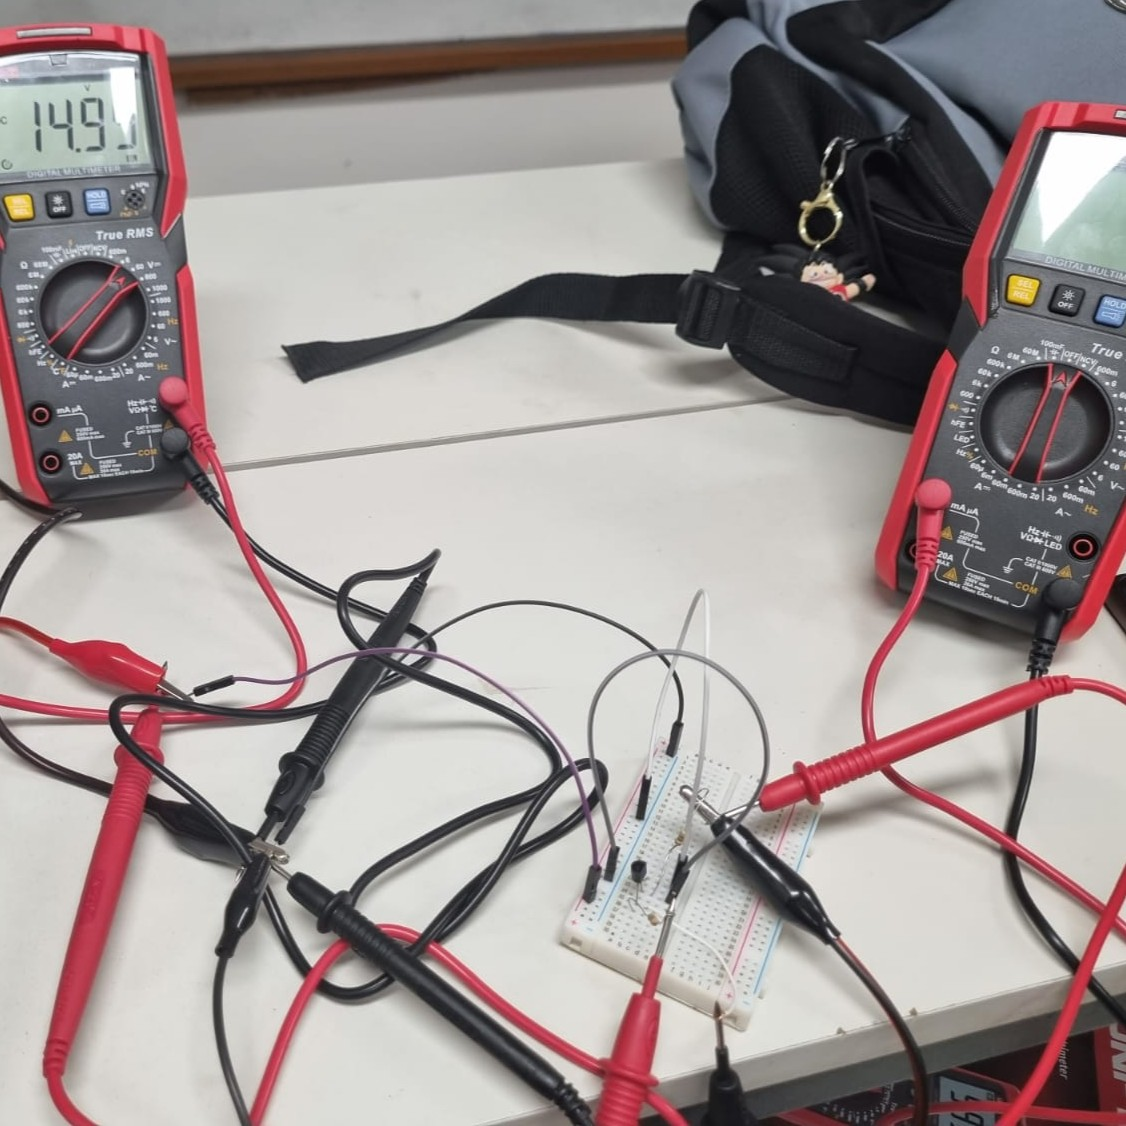
\includegraphics[width=6cm]{./imagenes/Lab2.jpg}

\begin{table}[ht]
\resizebox{6cm}{!}{%
\begin{tabular}{|l|l|}
\hline
\rowcolor[HTML]{FFCC67} 
$V_{GS}${[}mV{]} & $I_D${[}mA{]} \\ \hline
0                & 9,17          \\ \hline
36               & 8,57          \\ \hline
96,5             & 5,61          \\ \hline
172              & 4,06          \\ \hline
230              & 2,78          \\ \hline
265              & 2,46          \\ \hline
348              & 1,36          \\ \hline
396              & 0,86          \\ \hline
451              & 0,49          \\ \hline
537              & 0,21          \\ \hline
700              & 0,00124       \\ \hline
\end{tabular}%
}
\end{table}